%! TeX program = lualatex
\documentclass[../main.tex]{subfiles}
\begin{document}
\begin{lesson}{The Limit Laws}
  We learned how to estimate limits of functions. We now learn how to \hlsupp{evaluate} limits \emph{exactly}.

  % \faExclamationTriangle{} This section covers a bit more than the corresponding textbook section and is organized differently to minimize redundancy. See the last page for a short comparison.

  \begin{mdframed}[style=simple-compact]
    If a function \(f(x)\) is a polynomial or a rational function, then
    \[
      \lim_{x \to a} f(x) = f(a).
    \]
  \end{mdframed}
  \faExclamationTriangle{} Note \(a\) must be a constant \underline{\hspace{6cm}} and \underline{\hspace{2in}}.
  \blanklines{5}

  \begin{example}
    Evaluate \(\lim_{x \to -2} (x^{2} + 5 x^{3})\).

    \blanklines{5}
  \end{example}

  \begin{mdframed}[style=withref-compact]
    \textbf{Theorem} (Limit Laws). Suppose \(\lim_{x \to a} f(x)\) and \(\lim_{x \to a} g(x)\) {both exist}. Then
    \begin{enumerate}[label=(\arabic*)]
      \item \(\lim_{x \to a} [f(x) + g(x)] = \lim_{x \to a} f(x) + \lim_{x \to a} g(x)\) \hfill (sum)
      \item \(\lim_{x \to a} [f(x) - g(x)] = \lim_{t \to a} f(x) - \lim_{x \to a} g(x)\) \hfill (difference)
      \item \(\lim_{x \to a} [c \; f(x)] = c \lim_{t \to a} f(x)\), where \(c\) is a constant \hfill (constant multiple)
      \item \(\lim_{x \to a} [f(x) \; g(x)] = \lim_{x \to a} f(x) \cdot \lim_{x \to a} g(x)\) \hfill (product)
      \item \(\lim_{x \to a} \frac{f(x)}{g(x)} = \frac{\lim_{x \to a} f(x)}{\lim_{x \to a} g(x)}\), \quad if {\(\lim_{x \to a}g(x) \ne 0\)} \hfill (quotient)
      \item \(\lim_{x \to a} [f(x)]^{n} = \left[ \lim_{x \to a} f(x) \right]^{n}\) \hfill (power)
      \item \(\lim_{x \to a} \sqrt[n]{f(x)} = \sqrt[n]{\lim_{x \to a} f(x)}\), \quad if \(n\) is even, we assume {\(\lim_{x \to a} f(x) > 0\)} \hfill (root)
    \end{enumerate}
    \textbook{Theorem 2.5 Limit Laws on page 161}
  \end{mdframed}
  \faLightbulb{} Limit laws allow us to evaluate the limit of many algebraic functions \underline{\hspace{2in}}.
  % Before applying the limit laws, make sure the limit exists!

  % \begin{example}
  %   Evaluate \(\lim_{x \to 2} \left(\sin(x)\cos(x) - 2 e^{x} + \sqrt[3]{x}\right)\), if it exists.
  % \end{example}
  \clearpage

  Applying limit laws correctly is all about decomposing a function along algebraic operations to break up a larger task into smaller tasks. At the very end, we only evaluate limits of very simple functions such as polynomial and rational functions. The rest will be arithmetic.
  \begin{example}
    Let \(f(x) = \sqrt[5]{x^{2} + 1} - 2 (4x - 3)^{100}\). Evaluate \(\lim_{x \to 1} f(x)\).
    \blanklines{40}
  \end{example}
  \faExclamationTriangle{} As far as grading is concerned, we are expected to \hlwarn{show details of calculations} in assignments, tests and the final exam.  Unless stated otherwise, solutions (to short and long answer questions) without details or sufficient justification will typically be given \(0\), regardless of correctness. 
  \blanklines{5}

  Limit laws are still useful when only abstract information is given.
  \begin{example}
    Suppose \(\lim_{x \to -3} f(x) = 4\). Evaluate \(\lim_{x \to -3} \left( f(x) \right)^{3/2}\) if possible.
    \blanklines{10}
  \end{example}

  A variation-on-the-theme problem.  
  \begin{example}
    Let \(c\) be an unknown constant. Suppose \(\lim_{x \to 1} \sqrt{2x^{3} + cx - 1} = 3\). Find \(c\).
    \blanklines{10}
  \end{example}

  \faLightbulb{} Limit laws also apply to one-sided limits and piecewise functions.
  \begin{example}
    Let \(f(x) = \begin{cases}\sqrt{x - 1} + 1, &x > 1\\[1ex]\frac{2x}{x + 1}, &x < 1\end{cases}\). Evaluate \(\lim_{x \to 1} f(x)\).
    \blanklines{20}
  \end{example}
  \clearpage

  We now get into the more demanding territory of \hlmain{combining limit laws and algebra skills} to evaluate limits where the limit laws seemingly don't apply \hlsupp{at first glance}.

  \begin{example} \label{ex:limit-cancellation}
    Evaluate \(\lim_{t \to 2} \frac{t^{2} - 3t + 2}{t - 2}\) or explain why it does not exist.
    \blanklines{20}
  \end{example}

  \begin{example} \label{ex:limit-rationalization}
    Evaluate \(\lim_{x \to 0} \frac{\sqrt{x^{2}+1}-1}{x^{2}}\) or explain why it does not exist.
    \blanklines{20}
  \end{example}

  \faComment{} What exactly is going on in Example~\ref{ex:limit-cancellation} and \ref{ex:limit-rationalization}. Plot their graphs to find out!
  \clearpage

  Example~\ref{ex:limit-textbook-2.28} is a variation on the theme of Examples~\ref{ex:limit-cancellation} and \ref{ex:limit-rationalization} but challenges our algebra skills even more. It is a really good practice, but leave it until you have mastered all other skills. Hopefully, the hint at the bottom of the page helps.
  \begin{example}[Textbook Example~2.20] \label{ex:limit-textbook-2.28}
    Evaluate \(\lim_{x \to \infty} \frac{1}{x} + \frac{5}{x(x-5)}\) or explain why it does not exist.
    \blanklines{20}
  \end{example}

  Example~\ref{ex:limit-infinity-plus-constant} looks similar to Examples~\ref{ex:limit-cancellation} and \ref{ex:limit-rationalization} but is much simpler.
  \begin{example} \label{ex:limit-infinity-plus-constant}
    Evaluate \(\lim_{x \to 0^{-}} \frac{x+1}{x(x-1)}\) if it exists.
    \blanklines{18}
  \end{example}

  \vfill{}
  {\scriptsize Hint to Hint to Example~\ref{ex:limit-textbook-2.28}}. \newline
  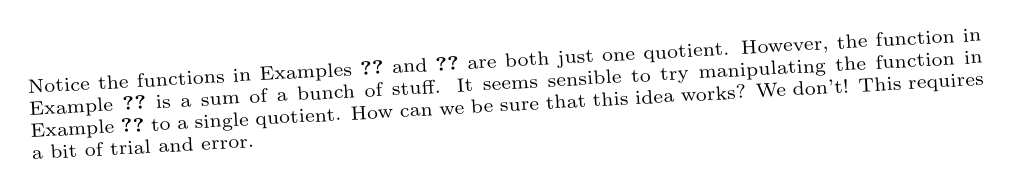
\begin{tikzpicture}[scale=1]
    \node[rotate={pi}, inner sep=0pt] {\parbox{\linewidth}{\scriptsize Notice the functions in Examples~\ref{ex:limit-cancellation} and \ref{ex:limit-rationalization} are both just one quotient. However, the function in Example~\ref{ex:limit-textbook-2.28} is a sum of a bunch of stuff. It seems sensible to try manipulating the function in Example~\ref{ex:limit-textbook-2.28} to a single quotient. How can we be sure that this idea works? We don't! This requires a bit of trial and error.}};
  \end{tikzpicture}
  \clearpage

  \begin{mdframed}[style=withref]
    \textbf{The Squeeze Theorem}. Let {\(f(x) \le g(x) \le h(x)\)} when \(x\) is near \(a\) (except possibly at \(a\)) and
    \[ { \lim_{x \to a} f(x) = \lim_{x \to a} h(x) = L,} \]
    then
    {\(\lim_{x \to a} g(x) = L\).}

    \textbook{\stewart{101}{\fbox{3} The Squeeze Theorem}}
  \end{mdframed}

  \begin{example}
    Evaluate \(\lim_{x \to 0} x \sin\left(\frac{1}{x}\right)\).

    \hfill\includegraphics[width=2in]{../standalones/build/plot_squeeze}
    \blanklines{30}
  \end{example}
  \clearpage

  \begin{example}
    Suppose \(x+1 \le h(x) \le x^{3} - 2x + 3\). Find \(\lim_{x \to 1} h(x)\).

    \blanklines{20}
  \end{example}
\end{lesson}
\end{document}

